
\section{Lightweight Audio Obfuscation}
\label{sec:obfuscation}

We require a lightweight obfuscation technique that can run in real-time on mobile devices with minimal computational effort.
 Driven by this constraint, I chose to explore two simple obfuscation techniques: decimation (downsampling/reducing the samplerate of audio) and imprecision (reducing the bit depth of the audio).
 Both these operations are quick and can run in real-time even in low-power microprocessors \footnote{One prevalent example of a low-power microprocessor that is ideal for this application is the Android Sensor Hub \cite{AndroidSensorHub}}.

\subsection{Decimation: Removing time fidelity}

If the audio stream is recorded at 16kHz, we decimate the audio stream to a much lower sampling frequency.
 With this operation, the intelligibility of speech rapidly decreases with the amount of decimation.
 However, this also significantly decreases keyword spotting performance \ref{sec:recognition_evaluation}.

\begin{gather}
\text{Decimate(Audio)} = \text{Downsample(Filter(Audio))}
\end{gather}

A Weiner filter is used here to process the audio.
 The Weiner filter works based on the probability of the sample belonging to the signal distribution or noise distribution.
 Therefore, it requires a specification of the noise power.
 The noise power is calculated as the variance of the first 100ms of recorded audio.
 The filter is applied in successive windows of 10ms of audio and the signal power is calculated as the variance of the audio window.

\begin{gather}
P(X[i:i+\text{window\_size}]) \sim \begin{cases}
  \mathcal{N}(0, \sigma_{\text{signal}}^2), \quad \mbox{if signal} \\
  \quad\quad\quad \text{\centering or,} \\
  \mathcal{N}(0, \sigma_{\text{noise}}^2), \quad \mbox{if noise}
 \end{cases}
\end{gather}

% \TODO{ some raw data vs subsampled data? and the FFT for both to visualize information loss?}

% \TODO{figure showing the performance decline of CMUSphinx, Google Speech Recog. with subsampled audio data}

% \TODO{discuss the entropy and information content after this operation with respect to the raw audio}

% \TODO{use differential privacy to discuss how adding controlled noise to this can prevent an attacker from understanding sensitive information.}


\subsection{Bit Depth: Removing amplitude fidelity}

If the audio stream is recorded at a 16-bit depth, we quantize the audio stream to a much lower bit depth to reduce the information content.
 Surprisingly, we find that, even at the lowest possible 1-bit depth, the speech content can be easily understood by humans (Figure \ref{fig:mturk_survey}).

% \TODO{discuss: the loss of information with quantization? not so much}

% \TODO{discuss the entropy and information content after this operation with respect to the raw audio}

% \TODO{use differential privacy to discuss how adding controlled noise to this can prevent an attacker from understanding sensitive information.}

\subsection{Obfuscating audio using hamming weights}

If we consider each audio sample as one "sample bit", then we can compute the hamming weight of $n$ sample bits.
 This is done by concatenating the sample bit strings and counting the total number of "1"s in the $n$-sample bit string.
 This operation increases the entropy of the obfuscated audio as compared to the original audio.
 A simpler way to analyze --- for a calculated hamming weight, there are combinatorially many possibilities for the "true" audio sample.
 The operation is illustrated in the example below. \\

\begin{tabular}{c}
\begin{tabular}{|C|C|C|C|}%
\hline%
\dots & 2919 & -32006 & \dots \\
\hline%
\multicolumn{4}{c}{which, in bit representation} \\
\hline%
\dots & 0000 \quad 1011 \quad 0110 \quad 0111 & 1000 \quad 0010 \quad 1111 \quad 1010 & \dots \\
\hline%
\end{tabular} \\
Audio Samples
\end{tabular} \\

If we apply hamming reduction on every 1 sample, \\

\begin{tabular}{c}
\begin{tabular}{|C|C|C|C|}%
\hline%
\dots & 8 & 8 & \dots \\
\hline%
\multicolumn{4}{c}{which, in bit representation} \\
\hline
\dots & 0000 \quad 0000 \quad 0000 \quad 1000 & 0000 \quad 0000 \quad 0000 \quad 1000 & \dots \\
\hline
\end{tabular} \\
Hamming Reduced Audio Samples (\texttt{hamming\_reduce\_1})
\end{tabular} \\

As we can see, although both the samples have extremely different values, but their hamming reductions are identical.
 For a hamming reduced value of $8$ the total number of possible "true" sample values with 16-bit audio are $16 \choose 8 = 12870$.
 Of course, the total number of possible "true" samples values decreases as the hamming value approaches $16$.
 More generally, the amount of privacy improvement resulting from the hamming operation can be defined as follows.


Let the reduced hamming weight value ($8$ in the example above) be represented by $R_s$.
 The number of sample-bits for the hamming operation ($1$ in the example above) is represented by $B_h$.
 The bit-depth of the audio ($16$ in the example above) is represented by $B_s$.

\begin{gather}
\text{Privacy Improvement from Hamming Reduction} = \frac{ {B_h \times B_s \choose R_s} - 1}{ 2^{(B_h \times B_s)} }
\end{gather}

Higher the order of the hamming operation, higher the privacy improvement.
 However, the hamming operation does decrease the performance of the classification of the deep learning model, so this is a trade-off that must be examined in detail.

% \TODO{discuss the entropy and information content after this operation with respect to the raw audio}

% \TODO{use differential privacy to discuss how adding controlled noise to this can prevent an attacker from understanding sensitive information.}

% \TODO{repeat the two analyses above applying the same hamming weight technique to both decimated audio and low bit-depth audio}

\subsection{Adding keywords to the dbHound system}

Training classification models for new keywords is quite straightforward using the existing dbHound framework \ref{sec:system_design}.
 To add a new set of keywords for the classification task, I propose a cascaded classification topology to avoid re-training older keyphrase models where the older keyphrases may be phonetically close to the newer keyphrase.


For example, if "hey savannah" is a new keyphrase --- since it sounds phonetically close to "hey cortana", a cascaded classification topology can be used.
 In the cascaded topology, the new keyphrase model is trained to classify all the original keyphrases as "random talk".
 Consequently, the newly trained model will be evaluated first (in the cascaded structure).
 If the audio does not belong to any of the new keyphrase model(s), then the audio is evaluated on the older keyphrase models to determine the class label.
 In a cascaded topology, this evaluation trickles down until the oldest keyphrase models are reached or until a keyphrase label with probability above the confidence threshold is found.
 This way, the computational expense in model evaluation is also minimized on average.

% \TODO{how would adding more keywords affect the privacy vs utility?}

% \TODO{can we say if we add keywords with certain characteristics the algorithm will still be fine?}


\subsection{Human-level performance}

Measuring Human level performance on a Deep Learning tasks is often an important metric and potentially leads to interesting insight \cite{NutsAndBoltsOfDL}.
 Following this paradigm, I selected 52 audio snippets from the TED-LIUM corpus \cite{TEDLIUMCorpus} and applied different levels of obfuscation using both the methods described above.
 Using workers from Amazon Mechanical Turk \cite{mturk}, the ability of humans to understand/decipher the speech content of obfuscated audio tracks was measured.
 The human transcription from the Mechanical Turk workers is compared against the original transcribed text in the TED-LIUM corpus to measure accuracy.
 The more accurate the transcription, the less effective the obfuscation technique.
 Surprisingly, I found that even when the bit-depth of audio is reduced to 1 bit, comprehensibility is quite high in most cases (the exception being audio with low Signal to Noise Ratio [SNR]).
 The results from the mechanical turk survey is shown in figure \ref{fig:mturk_survey}.
 The first 4 bars correspond to decreasing decimated frequencies.
 The last four bars correspond to decreasing bit depth of audio.

% \afterpage{
    \begin{figure}[H]
    \centering
    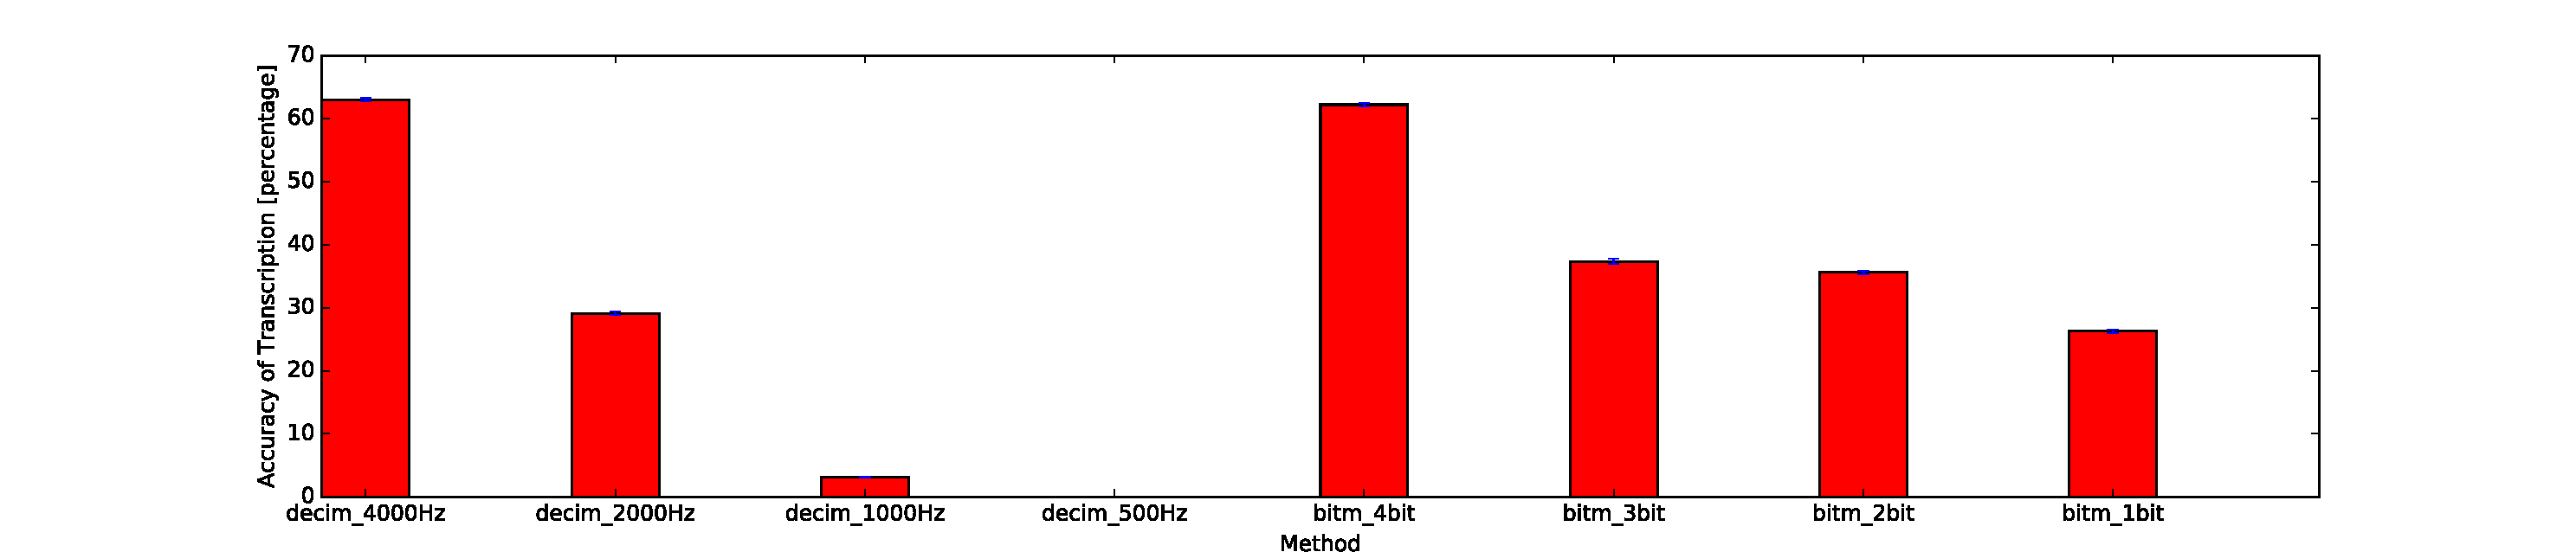
\includegraphics[width=\textwidth]{sound/mturk_survey.pdf}
    \caption{Accuracy of human transcription for different levels of decimation and quantization.}
    \label{fig:mturk_survey}
    \end{figure}
    \begin{table}[H]
    \begin{tabularx}{\textwidth}{l | l | l | l}
    \textbf{Key} & \textbf{Description} & \textbf{Key} & \textbf{Description} \\
    \hline
    decim\_4000 & Decimated to 4 kHZ & bitm\_4bit & 4-bit precision audio \\
    decim\_2000 & Decimated to 2 kHZ & bitm\_3bit & 3-bit precision audio \\
    decim\_1000 & Decimated to 1 kHZ & bitm\_2bit & 2-bit precision audio \\
    decim\_500 & Decimated to 500 HZ & bitm\_1bit & 1-bit precision audio \\
    \end{tabularx}
    \caption{Key for X-axis in Figure \ref{fig:mturk_survey}: \nameref{fig:mturk_survey}}
    \label{tab:key_mturk_survey}
    \end{table}
% }
% \clearpage

